\documentclass[11pt]{article}

\usepackage[preprint]{acl}

\usepackage{times}
\usepackage{latexsym}
\usepackage[T1]{fontenc}
\usepackage[utf8]{inputenc}
\usepackage[UTF8,fontset=none]{ctex}
\usepackage{microtype}
\IfFileExists{inconsolata.sty}{\usepackage{inconsolata}}{}

\usepackage{graphicx}
\usepackage{booktabs}
\usepackage{enumitem}
\usepackage{xspace}
\usepackage{amsmath}
\usepackage{amssymb}

\IfFontExistsTF{Droid Sans Fallback}{%
  \setCJKmainfont{Droid Sans Fallback}%
  \setCJKsansfont{Droid Sans Fallback}%
  \setCJKmonofont{Droid Sans Fallback}%
}{%
  \IfFontExistsTF{Songti SC}{%
    \setCJKmainfont{Songti SC}%
    \setCJKsansfont{Heiti SC}%
    \setCJKmonofont{STFangsong}%
  }{}%
}

\newcommand{\comve}{\textsc{ComVE}\xspace}
\newcommand{\taska}{Task A\xspace}
\newcommand{\method}{\textsc{LLM-CSR}\xspace}
\newcommand{\cmetric}[1]{\textsc{#1}}

\title{面向常识验证的大语言模型可靠性评估：鲁棒性、验证增强与不确定性分析}

\author{杨晨 \\
  复旦大学 \\ \And
  李威远 \\
  复旦大学 \\\And
  杨智超 \\
  复旦大学 \\}

\begin{document}
\maketitle

\begin{abstract}
常识验证要求模型判断一个自然语言陈述是否符合现实世界知识，是评估语言模型理解能力的重要任务。本文以 SemEval-2020 Task 4 \comve 子任务 A 为实验平台，研究大语言模型在两句相近文本中识别非常识句子的可靠性。除 RoBERTa 微调、零样本提示、少样本提示和自一致性等基础方法外，我们从两个互补方向扩展分析：一是评估模型在句子顺序、提示模板、少样本示例和采样随机性变化下的鲁棒性与一致性；二是探索 constraint-first prompting、generate-verify-rerank 和 consistency-based uncertainty 等轻量推理时增强方法。Task A 结果显示，RoBERTa 微调达到 0.868 准确率和 0.939 顺序一致性；最佳 LLM 为 Qwen3-1.7B thinking zero-shot direct prompt，准确率为 0.952，顺序一致性为 0.929，提示一致性为 0.849。8-shot 示例没有带来整体收益；no-thinking self-consistency 能将 Qwen3.5-2B minimal prompt 从 0.684 提升到 0.720，但仍低于 thinking zero-shot。Task B 结果显示，验证增强策略在 stronger models 上有进一步增益，例如 Qwen3.5-2B thinking 从 direct 的 0.782 提升到 rerank 的 0.818。整体来看，标准准确率不足以完整刻画大语言模型的常识能力；更可靠的常识验证还需要同时关注回答稳定性、解释是否支持判断，以及模型能否识别和利用自身不确定性。

\end{abstract}

\section{Introduction}

常识知识通常不会在文本中被显式说明，却是人类理解语言和判断事件可行性的基础。例如，把一只火鸡放进冰箱通常是合理的，而把一头大象放进冰箱则违反物体大小和容器容量之间的常识约束。对于大型语言模型而言，这类样本表面词汇相近、句式相似，但现实可行性完全不同，因此可以检验模型是否真正使用了稳定的世界知识，而不是依赖浅层词汇模式。

\comve 常识验证与解释任务由 Wang et al.~\citep{wang2019sensemaking,wang2020semeval} 提出并用于 SemEval-2020 Task 4。其中子任务 A 要求模型在两个相近句子中判断哪一个违背常识，是一个清晰、可复现的二分类任务。传统预训练编码器如 RoBERTa~\citep{liu2019roberta} 可以通过监督微调获得较强表现；近年来，大语言模型也能够通过提示学习、少样本学习和显式推理完成该任务。然而，仅报告一次性准确率并不能说明模型判断是否可靠。模型可能在原始测试集上表现较好，却对句子顺序、提示措辞、示例选择或采样随机性高度敏感。

近期研究也指出，常识推理和大语言模型可靠性需要从更细粒度角度评估。针对 \comve 的大语言模型评估发现，模型在验证任务上可能取得较高分数，但解释和稳定推理仍存在不足~\citep{comve_llm_2025}。HellaSwag-Pro 通过更困难和更多变的常识推理样本强调了题面扰动的重要性~\citep{hellaswagpro2025}。BrainBench 进一步显示，即使是强模型，在面向人类直觉的常识测试中仍会出现不稳定与退化~\citep{brainbench2026}。同时，test-time scaling 和自一致性研究表明，推理时多次采样、候选筛选和验证器重排可以在不重新训练模型的情况下改善部分推理任务~\citep{wang2023selfconsistency,testtime2025}。不确定性估计研究也表明，sample consistency 等黑盒置信度指标可用于分析 LLM 输出可靠性~\citep{uncertainty2025}。

本文将课程项目定位为常识验证中的大语言模型可靠性评估。我们保留 RoBERTa 微调和 LLM 提示式方法作为基础对照，同时设计两个并行扩展方向。第一个方向评估鲁棒性与一致性，关注输入扰动后模型答案是否保持等价。第二个方向研究验证增强与不确定性感知推理，关注模型能否通过显式常识约束、候选验证和采样一致性给出更可靠的判断。本文不加入中文翻译对比，因为当前数据集和官方任务均为英文，额外机器翻译会引入新的翻译质量变量，反而削弱对输入扰动和推理设置的聚焦。

本文的主要贡献体现在三个方面。首先，我们在 \comve 子任务 A 上构建 RoBERTa 与 Qwen 系列 LLM 的统一预测文件、指标文件和结果目录，并系统评估顺序交换、提示改写、少样本示例变化和采样随机性带来的鲁棒性问题。其次，我们探索 constraint-first、generate-verify-rerank 和 consistency uncertainty 等轻量推理时增强方法，观察它们是否能在不重新训练模型的情况下提升可靠性。最后，我们通过错误分析说明模型在物理常识、语言歧义、过度推理、prompt 敏感和高置信错误上的典型失败模式。

\section{Problem Definition}

\subsection{Task}

本文使用 SemEval-2020 Task 4 \comve 子任务 A。每个样本包含两个语义相近的英文句子：
\[
x = (\text{sent0}, \text{sent1})
\]
模型需要输出标签 \(y \in \{0,1\}\)，其中 \(0\) 表示 \texttt{sent0} 违背常识，\(1\) 表示 \texttt{sent1} 违背常识。

\subsection{Dataset}

官方数据集包含训练集、验证集和测试集。本文使用项目中预处理后的固定划分：训练集 10,000 条、验证集 1,000 条、测试集 1,000 条，且三个划分的标签均衡。所有方法使用相同数据划分，并以测试集准确率作为主要指标。8-shot 示例从训练集抽取，测试集只用于最终评估。

\subsection{Evaluation}

基础指标为准确率：
\[
\mathrm{Acc} = \frac{1}{N}\sum_{i=1}^{N}\mathbf{1}[\hat{y}_i = y_i].
\]

为刻画可靠性，本文进一步报告三类辅助指标。\cmetric{Order} 衡量交换 \texttt{sent0}/\texttt{sent1} 后模型预测是否同步翻转，用于判断模型是否理解标签与句子位置的对应关系；\cmetric{Prompt} 衡量同一样本在 direct、judge 和 minimal 三个语义等价 prompt 下预测是否一致，用于判断模型对提示措辞的敏感性；\cmetric{Sampling} 衡量 self-consistency 中同一 prompt 重复采样 5 次时多数标签所占比例，用于判断随机采样下输出是否稳定。

\section{Method}

\subsection{Supervised Baseline}

\paragraph{RoBERTa fine-tuning.}
RoBERTa 将 \texttt{sent0} 和 \texttt{sent1} 拼接为句子对输入，并在句子级表示上训练二分类头。该方法使用完整训练集，是本文的监督学习基线。测试时直接输出违反常识句子的索引，结果写入统一预测文件后再计算准确率和 order consistency。

\subsection{LLM Prompting}

\paragraph{Models and runtime.}
LLM 实验使用本地下载的 Qwen3-0.6B、Qwen3-1.7B、Qwen3.5-0.8B 和 Qwen3.5-2B。推理通过 vLLM 的 Python in-process API 完成，不使用 Transformers 逐条推理，也不启动 OpenAI 兼容服务。Qwen3.5 模型只用于文本输入输出，运行时关闭多模态路径。模型均比较 thinking 与 no-thinking 两种模式；最大输出长度按运行脚本固定为 no-thinking 10,240 tokens，thinking 16,384 tokens。

\paragraph{Prompt templates.}
每个样本使用三种英文提示模板：direct、judge 和 minimal。direct 模板直接要求选择违反常识的句子；judge 模板强调以严格裁判身份判断；minimal 模板仅保留最少任务说明。所有模板的最终答案均解析为标签 \(0/1\)。如果输出无法解析，则该条预测记为错误并保留 raw output 便于审计。

\paragraph{Zero-shot and 8-shot.}
Zero-shot 只提供任务说明和待判断句子。8-shot 在每个测试样本前加入 8 条训练集示例，示例标签保持平衡，用于检验上下文示例是否提升模型判断。本文不使用测试集选择示例或调参。

\subsection{Robustness and Consistency Tests}

\paragraph{Order swap.}
对测试集构造交换版本：交换 \texttt{sent0} 与 \texttt{sent1}，并将 gold label 翻转。若模型真正识别违反常识的语义内容，则原始样本和交换样本的预测也应同步翻转。本文同时报告交换后准确率和原/交换预测之间的 order consistency。

\paragraph{Prompt consistency.}
对同一样本比较 direct、judge 和 minimal 三个模板的预测是否一致。该指标不要求预测正确，只衡量模型在等价任务表述下是否稳定。因此它需要与准确率联合解释：高一致性可能来自稳定正确，也可能来自稳定偏置。

\paragraph{Self-consistency.}
为控制运行时间，self-consistency 只在 no-thinking 模式下运行 Qwen3-1.7B 和 Qwen3.5-2B，每个样本、每个模板重复采样 \(k=5\) 次，并使用多数投票得到最终标签。除多数投票准确率外，本文记录 sampling consistency，即 5 次采样中多数标签占比的平均值。

\subsection{Verification and Uncertainty Enhancements}

\paragraph{Constraint-first prompting.}
模型先抽取判断所需的常识约束，再分别检查两个句子，最后输出标签。该方法将任务拆成约束抽取与句子验证两个步骤，减少直接猜测标签的风险。

\paragraph{Generate-verify-rerank.}
模型首先生成多个候选答案和解释。随后使用 verifier 根据解释是否支持标签对候选进行评分，并选择分数最高的答案。该方法属于轻量 test-time scaling，不需要训练新模型。

\paragraph{Consistency-based uncertainty.}
对同一样本采样多次，用多数标签比例定义置信度：
\[
\mathrm{conf}(x)=\frac{\max_{y \in \{0,1\}}\sum_{j=1}^{k}\mathbf{1}[\hat{y}^{(j)}=y]}{k}.
\]
随后分析置信度与正确率的关系，并可进行 selective prediction：当 \(\mathrm{conf}(x)\) 高于阈值时才回答，否则标记为 uncertain。

\section{Experiments}

\subsection{Experimental Setup}

\paragraph{Models.}
本文比较 RoBERTa 微调模型与 4 个本地 Qwen 小模型：Qwen3-0.6B、Qwen3-1.7B、Qwen3.5-0.8B 和 Qwen3.5-2B。所有 LLM 实验均在同一份 \comve Task A test 集上运行，并分别测试 no-thinking 与 thinking 两种推理模式。Task B 在相同模型集合上进一步评估 direct prompting、constraint-first prompting 与 generate-verify-rerank 三种 test-time enhancement 策略。

\paragraph{Prompts and outputs.}
Task A 使用 direct、judge 和 minimal 三种 prompt 模板；8-shot 设置在同一测试集上加入 8 个固定训练示例；self-consistency 设置对每个样本和模板重复采样 5 次并做多数投票。实验使用项目内固定测试集，共 1,000 条样本。Task B 在同一测试集上复用 direct baseline，并额外比较 constraint-first 与 generate-verify-rerank。两个方向的输出都写入项目的 results 目录；报告正文只引用汇总指标，复现入口和文件组织放在附录说明。

\paragraph{Metrics.}
主实验报告 accuracy；鲁棒性实验报告 order consistency、prompt consistency 和 sampling consistency。Order consistency 衡量交换两个候选句顺序后模型预测是否同步翻转；prompt consistency 衡量同一模型在三种模板下预测是否一致；sampling consistency 衡量重复采样的多数标签占比。Task B 报告不同推理增强策略的最终 accuracy，并用折线图比较模型规模与推理模式的关系。

\paragraph{Completeness check.}
Task A vLLM 实验覆盖 zero-shot、8-shot、order swap 和 self-consistency；Task B 实验覆盖 direct、constraint-first 和 rerank。两部分都以同一测试集大小作为基本校验，预测文件和指标文件均通过行数检查。

\subsection{Task A Main Results}

\begin{table}[t]
\centering
\small
\resizebox{\linewidth}{!}{%
\begin{tabular}{lccc}
\toprule
Method & Acc. & Consistency & Notes \\
\midrule
RoBERTa fine-tuning & 0.868 & Order 0.939 & supervised \\
Qwen3-1.7B zero-shot & \textbf{0.952} & Prompt 0.849 / Order 0.929 & thinking, direct \\
Qwen3-1.7B 8-shot & 0.931 & Prompt 0.849 & thinking, direct \\
Qwen3.5-2B self-consistency & 0.720 & Prompt 0.550 / Sampling 0.794 & no-thinking, minimal \\
\bottomrule
\end{tabular}%
}
\caption{\comve Task A 主结果。Acc. 为测试集准确率；Consistency 列报告该设置下最相关的一致性指标。}
\label{tab:main_results}
\end{table}

表~\ref{tab:main_results} 显示，最佳 LLM 设置显著超过 RoBERTa：Qwen3-1.7B thinking zero-shot direct prompt 达到 0.952 准确率，比 RoBERTa 高 8.4 个百分点。同时，该设置的 order consistency 为 0.929，接近 RoBERTa 的 0.939，说明高准确率并非完全来自位置偏置。8-shot 没有提升最佳 direct prompt，反而从 0.952 降至 0.931。No-thinking self-consistency 的最佳结果为 Qwen3.5-2B minimal prompt，准确率 0.720，低于 thinking zero-shot，但高于同模型 no-thinking zero-shot minimal prompt 的 0.684。

\subsection{Task A Zero-shot Results}

本小节单独展开 zero-shot，是因为它构成后续 few-shot、self-consistency 与 Task B direct baseline 的参照点。表~\ref{tab:zero_results} 汇总每个代表模型和推理模式下的最佳 prompt，可以看到 thinking 模式在所有强模型上都明显占优；no-thinking 设置虽然偶尔能通过 minimal prompt 获得可用结果，但整体上仍低于对应 thinking 版本。

\begin{table}[t]
\centering
\small
\resizebox{\linewidth}{!}{%
\begin{tabular}{llcc}
\toprule
Model & Setting & Best prompt & Acc. \\
\midrule
Qwen3-1.7B & thinking & direct & \textbf{0.952} \\
Qwen3-0.6B & thinking & minimal & 0.819 \\
Qwen3.5-2B & thinking & direct & 0.803 \\
Qwen3.5-0.8B & thinking & direct & 0.724 \\
Qwen3-1.7B & no-thinking & minimal & 0.706 \\
Qwen3.5-2B & no-thinking & minimal & 0.684 \\
\bottomrule
\end{tabular}%
}
\caption{Zero-shot 设置下每个代表模型/模式的最佳 prompt。Thinking 模式整体优于 no-thinking。}
\label{tab:zero_results}
\end{table}

从 prompt 角度看，direct prompt 对 Qwen3-1.7B 和 Qwen3.5-2B thinking 最有效，而 minimal prompt 对 Qwen3-0.6B thinking 与 no-thinking 模型更稳。这说明不同规模模型对指令复杂度的偏好并不相同：较强模型能够利用更明确的判断指令，较弱模型则更容易从短 prompt 中受益。这个观察也解释了为什么后续 Task B 不只比较最终 accuracy，还需要比较 direct、constraint-first 和 rerank 三种推理形式。

\subsection{Task A Robustness Results}

\begin{table}[t]
\centering
\small
\resizebox{\linewidth}{!}{%
\begin{tabular}{lcccc}
\toprule
Method & Acc. & Swap Acc. & Order & Prompt \\
\midrule
RoBERTa fine-tuning & 0.868 & 0.867 & \textbf{0.939} & -- \\
Qwen3-1.7B thinking direct & \textbf{0.952} & \textbf{0.949} & 0.929 & \textbf{0.849} \\
Qwen3-1.7B thinking judge & 0.938 & 0.932 & 0.908 & \textbf{0.849} \\
Qwen3-1.7B thinking minimal & 0.885 & 0.888 & 0.811 & \textbf{0.849} \\
Qwen3.5-2B thinking direct & 0.803 & 0.784 & 0.691 & 0.461 \\
Qwen3.5-2B thinking minimal & 0.800 & 0.786 & 0.676 & 0.461 \\
\bottomrule
\end{tabular}%
}
\caption{顺序交换与提示一致性结果。Swap Acc. 是交换句子顺序后的准确率；Order 是原始预测与交换预测是否同步翻转。}
\label{tab:robustness_results}
\end{table}

表~\ref{tab:robustness_results} 中，Qwen3-1.7B thinking 不仅准确率最高，而且在三种 prompt 上都保持较高顺序一致性。相比之下，Qwen3.5-2B thinking 的准确率仍可达到 0.800 左右，但 order consistency 降至 0.676--0.691，说明它对句子位置和 prompt 形式更敏感。若再看 sampling consistency，Qwen3-1.7B thinking 的多数标签占比为 0.888，明显高于对应 no-thinking 设置，说明其多次采样时的决策边界也更稳定。

\subsection{Few-shot and Self-consistency}

\begin{table}[t]
\centering
\small
\resizebox{\linewidth}{!}{%
\begin{tabular}{llccc}
\toprule
Model & Prompt & Zero-shot & 8-shot & Delta \\
\midrule
Qwen3-1.7B thinking & direct & 0.952 & 0.931 & -0.021 \\
Qwen3-1.7B thinking & judge & 0.938 & 0.920 & -0.018 \\
Qwen3-1.7B thinking & minimal & 0.885 & 0.891 & +0.006 \\
Qwen3.5-2B thinking & direct & 0.803 & 0.500 & -0.303 \\
Qwen3-0.6B thinking & minimal & 0.819 & 0.607 & -0.212 \\
\bottomrule
\end{tabular}%
}
\caption{8-shot 与 zero-shot 的比较。少样本示例并未稳定提升，部分模型明显退化。}
\label{tab:fewshot_results}
\end{table}

\begin{table}[t]
\centering
\small
\resizebox{\linewidth}{!}{%
\begin{tabular}{llccc}
\toprule
Model & Prompt & Acc. & Prompt & Sampling \\
\midrule
Qwen3.5-2B no-thinking & minimal & \textbf{0.720} & 0.550 & 0.794 \\
Qwen3-1.7B no-thinking & minimal & 0.701 & 0.252 & \textbf{0.970} \\
Qwen3.5-2B no-thinking & direct & 0.568 & 0.550 & 0.767 \\
Qwen3-1.7B no-thinking & direct & 0.563 & 0.252 & 0.967 \\
\bottomrule
\end{tabular}%
}
\caption{No-thinking self-consistency，采样次数 $k=5$。Sampling 是多数标签占比的平均值。}
\label{tab:self_consistency_results}
\end{table}

表~\ref{tab:self_consistency_results} 表明，采样一致性不能直接等同于正确性。Qwen3-1.7B no-thinking minimal prompt 的 sampling consistency 高达 0.970，但准确率只有 0.701；Qwen3.5-2B no-thinking minimal prompt 的采样一致性较低，却获得更高准确率 0.720。

\subsection{Task B Main Results}

Task B 的目标不是重新设计数据集，而是在 Task A 的二分类常识验证框架上测试推理时增强是否有额外收益。因此表~\ref{tab:verification_results} 采用与 Task A 主表相同的读法：先看 direct baseline，再比较增强策略相对 direct 的变化。Task B direct 与 Task A direct 基本处于同一数量级，说明两个方向在输出约束对齐后具有可比性。

\begin{table*}[t]
\centering
\small
\setlength{\tabcolsep}{4.5pt}
\begin{tabular}{llrrrr}
\toprule
Model & Mode & Task A Direct & Task B Direct & Constraint & Rerank \\
\midrule
Qwen3-0.6B & no-think & 0.500 & 0.500 & 0.500 & 0.434 \\
Qwen3-1.7B & no-think & 0.565 & 0.574 & 0.504 & 0.737 \\
Qwen3.5-0.8B & no-think & 0.470 & 0.466 & 0.478 & 0.500 \\
Qwen3.5-2B & no-think & 0.566 & 0.572 & 0.560 & 0.602 \\
Qwen3-0.6B & think & 0.709 & 0.682 & 0.694 & 0.712 \\
Qwen3-1.7B & think & 0.952 & 0.941 & 0.946 & 0.950 \\
Qwen3.5-0.8B & think & 0.724 & 0.691 & 0.703 & 0.721 \\
Qwen3.5-2B & think & 0.803 & 0.782 & 0.795 & 0.818 \\
\bottomrule
\end{tabular}
\caption{Task B 主结果。Task A Direct 是同模型 direct prompt 的参照基线；其余三列为 Task B 中的 direct、constraint-first 和 generate-verify-rerank。}
\label{tab:verification_results}
\end{table*}

表~\ref{tab:verification_results} 中的整体排序与 Task A 保持一致：Qwen3-1.7B thinking 仍然最强，Qwen3.5-2B thinking 次之，小模型和 no-thinking 设置明显更不稳定。这种一致性很重要，因为它说明 Task B 的增强流程没有引入一个完全不同的评估问题，而是在同一常识验证能力上观察 test-time inference 的边际收益。

\subsection{Task B Strategy Comparison}

从策略对比看，constraint-first 的收益依赖模型是否具备足够稳定的中间推理能力。在 thinking 模式下，它通常略高于 direct，例如 Qwen3-1.7B 从 0.941 提升到 0.946，Qwen3.5-2B 从 0.782 提升到 0.795；但在 no-thinking 模式下，constraint-first 对小模型帮助有限，甚至可能因为中间链条更长而扩大错误传播。

Generate-verify-rerank 的作用更接近对候选解释的筛选。强模型 direct 阶段已经能做出较优判断，因此 rerank 的提升较小但方向稳定；中强模型的收益更明显，例如 Qwen3.5-2B thinking 从 constraint-first 的 0.795 进一步提升到 0.818。相反，对于基础推理能力不足的模型，候选生成本身质量不稳定，verifier 能筛出的有效信息有限。

\subsection{Task B Figure Analysis}

\begin{figure}[t]
\centering
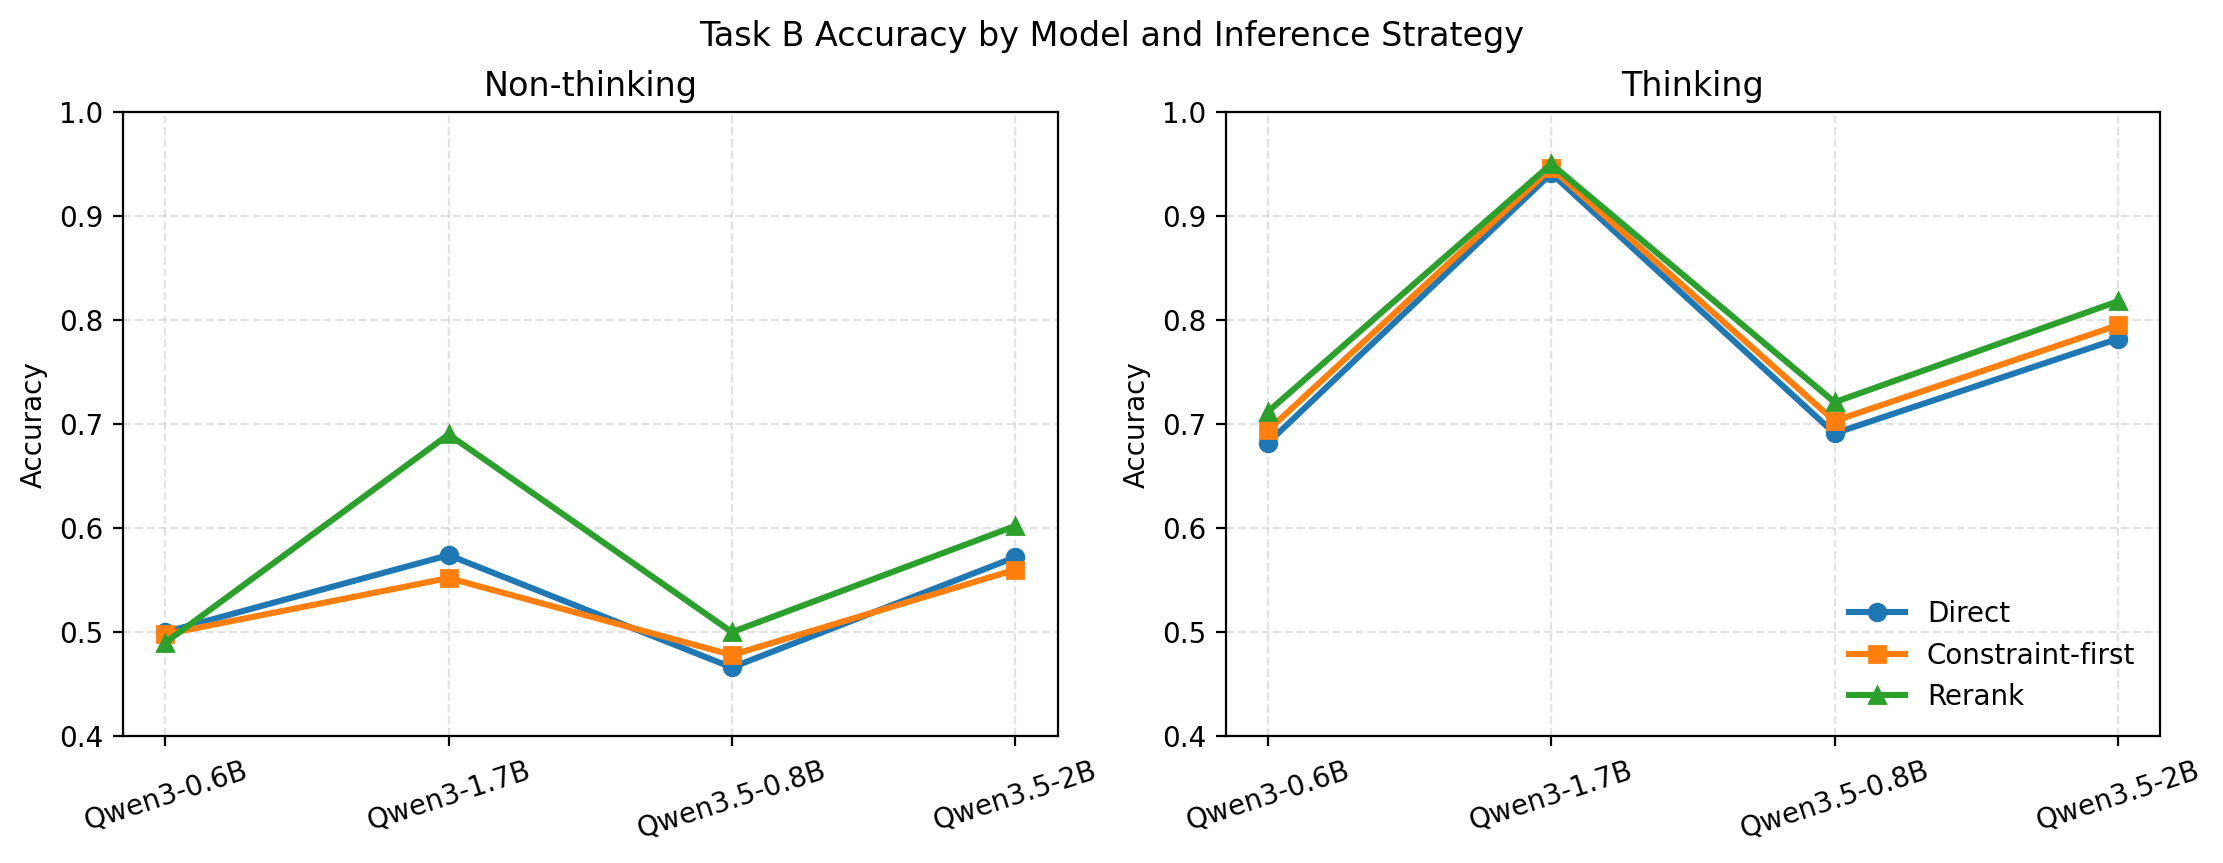
\includegraphics[width=\linewidth]{figures/task_b_accuracy_lines.png}
\caption{Task B 中不同推理策略随模型规模变化的准确率折线图。左图为 no-thinking，右图为 thinking。可以看到 thinking 模式下三条曲线整体上移，而 rerank 曲线在 stronger models 上与其他方法拉开更明显差距。}
\label{fig:taskb_accuracy_lines}
\end{figure}

图~\ref{fig:taskb_accuracy_lines} 将表格中的趋势可视化。左侧 no-thinking 曲线波动较大，说明在基础推理不稳定时，增加 constraint 或 verifier 不一定可靠；右侧 thinking 曲线整体上移，并且 direct、constraint、rerank 的相对顺序更清晰。由此可以把 Task B 的结论概括为：推理时增强更像能力放大器，而不是能力替代器；它最适合已经具备较强常识判断能力、但仍会在边界样本上摇摆的模型。

\section{Analysis}

\subsection{Error Taxonomy}

本文从测试集中错误样本的典型现象出发，将失败模式归纳为五类。第一类是 physical commonsense，即物体大小、空间容量、时间顺序或生理约束判断错误。第二类是 lexical ambiguity，即关键词存在歧义，模型误解句子含义。第三类是 over-reasoning，即模型引入题面没有给出的额外假设。第四类是 prompt sensitivity，即不同 prompt 导致不同标签。第五类是 high-confidence errors，即多次采样高度一致但最终错误。

\subsection{Task A: Accuracy Is Not Enough}

RoBERTa 与 Qwen3-1.7B thinking 的对比说明，准确率和鲁棒性需要同时看。RoBERTa 的准确率为 0.868，低于最佳 LLM，但 order consistency 达到 0.939，是所有方法中最高。这说明监督分类器虽然能力上限较低，但对句子交换扰动非常稳定。Qwen3-1.7B thinking direct prompt 的准确率达到 0.952，order consistency 也有 0.929，因此它是本文最可靠的单一设置。相反，Qwen3.5-2B thinking minimal prompt 的准确率为 0.800，但 order consistency 只有 0.676，说明其一部分正确答案可能依赖原始输入格式。

从 zero-shot 结果看，thinking 模式是性能提升的主要来源。Qwen3-1.7B 在 thinking direct prompt 下达到 0.952，而 no-thinking 最佳 prompt 只有 0.706。Qwen3.5-2B thinking 的 direct/minimal prompt 分别达到 0.803/0.800，也明显高于 no-thinking zero-shot minimal prompt 的 0.684。这个结果符合常识验证任务的性质：两个句子通常只差一个关键事件约束，模型需要比较物理可行性、时间关系或社会常识，而不仅是识别表面词。

如果再看 sampling consistency，Qwen3-1.7B thinking 的多数标签占比也明显高于 no-thinking 版本，说明更强的模型不仅更容易在单次推理中答对，也更能在多次随机采样时维持相对稳定的决策边界。这一点对后续的 self-consistency 或 rerank 策略尤其重要，因为它意味着模型的可投票性本身就更强。

\subsection{Few-shot and Self-consistency}

8-shot 结果没有稳定提升。最佳 Qwen3-1.7B thinking direct prompt 从 0.952 降至 0.931，judge prompt 从 0.938 降至 0.920，仅 minimal prompt 从 0.885 小幅升至 0.891。更明显的是，Qwen3.5-2B thinking direct prompt 从 0.803 降至 0.500，接近随机水平。这说明少样本示例会改变模型对输出格式和判断线索的关注方式；在本任务中，少样本上下文并不自动优于简洁 zero-shot 指令。

No-thinking self-consistency 的结果说明，多次采样多数投票可以提升部分设置，但无法替代 thinking 推理。Qwen3.5-2B no-thinking minimal prompt 从 zero-shot 的 0.684 提升到 self-consistency 的 0.720，说明多数投票能减少一部分随机错误。然而，Qwen3-1.7B no-thinking minimal prompt 的 sampling consistency 达到 0.970，准确率只有 0.701。这类结果是稳定但不够正确的典型例子：模型多次采样高度一致，但一致性主要反映固定偏置，而不是可靠常识判断。

\subsection{Task B: Verification as an Amplifier}

Task B 的结果更直接地回答了推理时增强是否真正提升可靠性这一问题。首先，direct prompting 在两种推理模式下都与 Task A direct baseline 保持接近，说明 Task B 新增的验证流程并没有改变模型的基础难度排序。其次，constraint-first prompting 对 stronger models 更有效：Qwen3-1.7B 与 Qwen3.5-2B 在 thinking 模式下都出现了稳定提升，而 Qwen3-0.6B 与 Qwen3.5-0.8B 的提升幅度较小，说明先抽取 commonsense constraints 再做判断，需要模型本身具备足够稳定的中间推理能力。

Generate-verify-rerank 的整体表现也符合这一规律。对于 no-thinking 模型，rerank 的收益不稳定，有时仅有小幅提升；但在 thinking 模式下，四个模型都出现了进一步改善，并且提升幅度与模型基础能力相关。Qwen3-1.7B 的 direct、constraint 与 rerank 分别为 0.941、0.946 和 0.950，说明强模型本身已经能在 direct 阶段做出较优决策，rerank 更多是在边界样本上做细化筛选。相比之下，Qwen3.5-2B 从 0.782 提升到 0.818，说明中强模型更能受益于先生成多个解释再用 verifier 重排的策略。

从整体趋势看，Task B 的主要价值不是把弱模型突然抬到很高水平，而是在保持与 Task A 一致的能力排序前提下，进一步提高 stronger models 的决策稳定性与最终准确率。换言之，verification-enhanced inference 更像是一种能力放大器，而不是能力替代器：它对基础能力较强、能稳定生成高质量候选解释的模型更有效，而对基础推理较弱的模型收益有限。

\subsection{Case Study Directions}

每个案例可包含原始句子、gold label、模型预测、模型解释、扰动后预测和错误类型。本文重点讨论三类代表性案例。

\paragraph{Case 1: constraint-first 修正 direct 的边界样本。}
一个典型例子是涉及用途与对象匹配的样本，例如卡车可以用来拖设备或船只，而船只会拖卡车。在这类样本上，direct prompting 往往只依赖局部搭配熟悉度做快速判断，而 constraint-first prompting 会先显式写出运输工具的典型承载方向、船通常被卡车运输而不是反向运输等 commonsense constraints，因此更容易把错误定位到第二句。该现象解释了为什么 stronger models 在 thinking 模式下能从 constraint-first 中获得稳定增益。

\paragraph{Case 2: rerank 修正 lexical ambiguity。}
另一类案例出现在词汇搭配本身合理、但真实世界关系错误的样本中。例如他打开了桌子和他打开了灯这类 pair，direct prompting 容易被打开这一高频动词带偏，而 candidate generation 往往会产生多个解释版本，其中一部分会明确指出桌子通常不具备可被打开的开关属性。在这类样本上，verifier 的作用不是创造新知识，而是把更符合世界知识的候选解释排到前面，因此 rerank 会优于单次 direct 决策。

\paragraph{Case 3: high-confidence but wrong。}
第三类失败案例出现在人物属性或动机推断上，例如一个勤奋的人整天学习与一个勤奋的人整天打手机游戏。这类样本的冲突不涉及明显物理常识，而是依赖对人物特质和行为倾向的社会常识判断。模型即使在 thinking 模式下也可能给出结构完整、语气自信的解释，但仍把勤奋错误泛化为任何持续行为都可被解释为努力。这类错误说明，高置信并不一定意味着真正掌握了正确规则，也是 selective prediction 和 uncertainty analysis 需要重点关注的对象。

\section{Conclusion}

本文围绕 \comve 常识验证任务系统评估了大语言模型的判断可靠性。Task A 结果显示，RoBERTa 微调基线达到 0.868 准确率和 0.939 顺序一致性；最佳 LLM 设置为 Qwen3-1.7B thinking zero-shot direct prompt，准确率达到 0.952，order consistency 为 0.929，prompt consistency 为 0.849。8-shot 示例没有带来稳定收益，self-consistency 在 no-thinking 模式下只能有限改善部分模型，仍无法超过 thinking zero-shot。Task B 结果显示，verification-enhanced inference 在 stronger models 上还能带来进一步收益，尤其是 Qwen3.5-2B thinking 的 rerank 准确率达到 0.818。总体而言，标准准确率只能回答模型是否答对，而鲁棒性与不确定性分析进一步回答模型是否稳定地答对以及是否知道自己可能答错。这为常识验证中的大语言模型评估提供了比单一 baseline 比较更完整的研究叙事。


\bibliography{reference}

\appendix
\section{实现细节与复现说明}

\subsection{提示模板}

\paragraph{Direct prompting.}
Direct prompt 要求模型直接完成二分类常识验证，并且最终只返回一个标签。核心指令是：给定 Sentence 0 和 Sentence 1，如果 Sentence 0 违背常识则输出 0，如果 Sentence 1 违背常识则输出 1。该格式用于 Task A，也作为 Task B 的 direct baseline。

\paragraph{Judge prompt.}
Judge prompt 将模型设定为严格常识裁判，要求它阅读两个句子并判断哪一个句子不可能或违背常识，最后只返回该句子的索引。该模板用于测试模型是否会因为任务措辞更强调裁判角色而改变预测。

\paragraph{Minimal prompt.}
Minimal prompt 只保留最短任务说明，即询问哪一个句子违背常识，并要求回答 0 或 1。它用于测试模型在低约束提示下是否仍能保持稳定输出。

\paragraph{Constraint-first prompting.}
Constraint-first prompting 要求模型先写出判断句子对所需的常识约束，再分别检查两个句子是否违反该约束，最后输出单个标签。最终评估只使用解析出的标签计算 accuracy，中间解释保留用于定性分析。

\paragraph{Verifier prompt.}
Verifier prompt 接收原始句子对和一个候选答案，要求模型判断候选解释是否支持该标签，并返回 1 到 5 的分数以及最终标签。Generate-verify-rerank 使用该分数选择最终预测。

\subsection{预测文件格式}

所有预测文件使用统一 CSV 格式：
\[
\texttt{id, method, pred, gold, correct, notes}.
\]
\texttt{id} 表示测试样本编号，\texttt{method} 记录模型和提示策略，\texttt{pred} 与 \texttt{gold} 分别表示预测标签和真实标签，\texttt{correct} 是二值正确性标记。\texttt{notes} 字段保存额外元数据，例如采样编号、verifier score、confidence 或解析状态。

\subsection{复现实验入口}

Task A 的数据验证、RoBERTa 训练、vLLM 推理、8-shot、order swap 和 self-consistency 结果整理位于 \texttt{task\_a\_robustness} 包及相关脚本中。Task B 的 prompt 生成、response 解析、verifier prompt 构造、rerank 和 uncertainty analysis 位于 \texttt{task\_b\_verification\_uncertainty} 包中。Task B 的批量运行入口由 verification pipeline 脚本和 uncertainty 脚本提供。

\subsection{结果文件}

Task A 的 RoBERTa 结果保存在 \texttt{results/task\_a/roberta/}，Task A 的 vLLM 结果保存在 \texttt{results/task\_a/vllm/}，报告表格保存在 \texttt{results/task\_a/report\_tables/}。Task B 的验证增强结果保存在 \texttt{results/task\_b/vllm/}。报告中的表格均由这些 CSV 文件整理得到，图~\ref{fig:taskb_accuracy_lines} 由 Task B accuracy 汇总结果生成。


\end{document}
